\documentclass[tikz]{standalone}
\usepackage{pgfplots}
\usepackage{xcolor} % For using hex colors
\usetikzlibrary{calc}
\definecolor{mycolor}{HTML}{ffd966} % Define custom color #ffd966
\pgfplotsset{compat=1.18}

\begin{document}
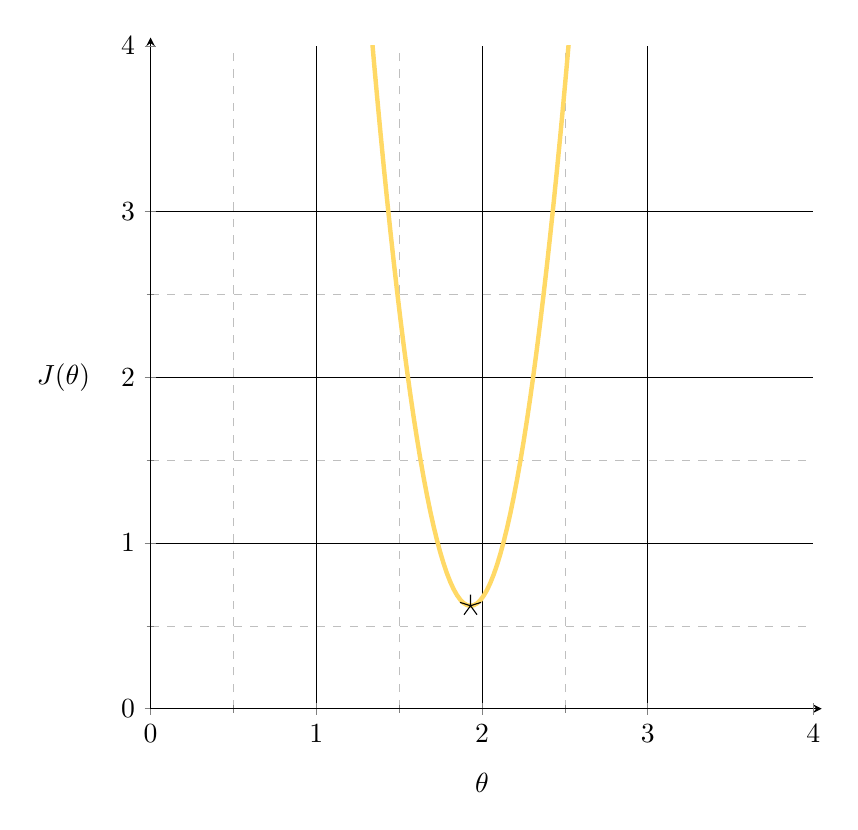
\begin{tikzpicture}
  \begin{axis}[
    % Draw only the bottom and left axes with arrow tips:
    axis lines=left,
    x axis line style={->,>=stealth, shorten >=-3pt},
    y axis line style={->,>=stealth, shorten >=-3pt},
    xlabel={\(\theta\)},
    ylabel={\(J(\theta)\)},
    % Rotate the y label so that it appears upside down:
    ylabel style={rotate=-90},
    xmin=0, xmax=4,
    ymin=0, ymax=4,
    % Major ticks at integer values (0 to 3)...
    xtick={0,1,...,3},
    ytick={0,1,...,3},
    % ...and an extra tick at 4 (without grid lines):
    extra x ticks={4},
    extra x tick style={grid=none},
    extra y ticks={4},
    extra y tick style={grid=none},
    % One minor tick (at 0.5) between each major tick:
    minor x tick num=1,
    minor y tick num=1,
    grid=both,
    % Grid styling:
    major grid style={line width=0.2pt,draw=black},
    minor grid style={line width=0.1pt,draw=gray!50,dashed},
    width=10cm,
    height=10cm,
  ]
    % Plot the function 
    % f(θ) = 1/3[(2θ-5)^2 + (3θ-6)^2 + (4θ-7)^2]
    \addplot[domain=0:4, samples=200, ultra thick, color=mycolor] 
      {((2*x-5)^2 + (3*x-6)^2 + (4*x-7)^2)/3};
    % Tangent line at θ=2.5. J(2.5)=3.75 and J'(2.5)=11 → y = 11(x-2.5)+3.75
    \addplot[domain=0:4, samples=2, thick, color=mycolor, restrict y to domain=0:4]
      {11*(x-2.5)+3.75};
    
    % Mark the minimum point (θ ≈ 1.931, f(θ) ≈ 0.621) with a red star:
    \addplot[only marks, mark=star, mark options={scale=2, fill=red}] 
    coordinates {(1.931,0.621)};
  \end{axis}
\end{tikzpicture}
\end{document}